\documentclass[12pt,a4paper]{article}
\usepackage{amsmath, amssymb}
\usepackage{geometry}
\usepackage{hyperref}
\usepackage{booktabs}
\usepackage{graphicx}
\usepackage{setspace}
\graphicspath{{assets/}}

%title page
\geometry{margin=1in}

\begin{document}

% Title Page
\begin{titlepage}
    \centering
    
    \Huge
    \textbf{Jaypee Institute of Information Technology, Sector - 62, Noida } \\
    \vspace{0.5cm}
    \Large
    \textbf{B.Tech CSE I Semester}\\
    \vspace{1cm}
    \vspace*{\fill}
    
    
\includegraphics[scale=0.2]{jiit_logo}\\
    
    \vspace{1.5cm}
    \Huge
    \textbf{Physics PBL Report}\\
    \Large
    
    \textbf{Einstein's General Relativity}\\
    \vspace{1cm}

    \Large
    \textbf{Submitted to}\\
    Dr. Sandeep Mishra
    \vspace{1cm}

    \textbf{Submitted by}
    \vspace{0.5cm}

    \begin{tabular}{ll}
        Harsh Sharma & 2401030232 \\
        Karvy Singh & 2401030234 \\
    \end{tabular}

    \vspace*{\fill}
    \normalsize
\end{titlepage}

%letter of transmittal 
\begin{center}
    \Large\textbf{Letter of Transmittal}
\end{center}
\vspace{1cm}

\noindent
\textbf{Dr. Sandeep Mishra} \\
[0.5em]
Department of Physics and Materials Science and Engineering\\
[0.5em]
% University/Institute Name \\
% [Address] \\

\vspace{1cm}

\noindent
\textbf{Subject:} Submission of Report on ``Einstein's General Relativity''

\vspace{1cm}

\noindent
Dear Dr. Sandeep Mishra,

\vspace{1em}

\noindent
We are pleased to submit our report titled \textit{``Einstein's General Relativity''} as part of our coursework. This report explores the mathematical foundations of General theory of Relativity, focusing on explaining how the aspect of Einstein's theory for black holes was wrong, its mathematical aspects and their relation with existance of Blackholes, Whiteholes and Wormholes.

\vspace{1em}

\noindent
We have endeavored to cover the theoretical aspects comprehensively and hope that this report meets your expectations.

\vspace{1em}

\noindent
Thank you for your guidance and the opportunity to work on this project.

\vspace{2em}

\noindent
Sincerely, \\[2em]

\noindent
Harsh Sharma (2401030232)\\
Karvy Singh (2401030234)\\

\vspace{2cm}

\noindent
Date: \today

\newpage

\tableofcontents

\newpage

\section{Introduction}
Gravity, one of the fundamental forces of nature, governs the motion of planets, stars, and galaxies, shaping the very fabric of the universe. From Isaac Newton’s classical description of gravitational attraction to Albert Einstein’s revolutionary concept of spacetime curvature, our understanding of gravity has evolved significantly over the centuries. Among the most intriguing consequences of this evolution is the existence of black holes—regions in space where gravity is so intense that not even light can escape.


Black holes are more than just cosmic curiosities; they are key to understanding the nature of spacetime, the lifecycle of stars, and the interplay between gravity and matter under extreme conditions. This text delves into the mechanics of gravity, the formation of black holes by relating it to General theory of relativity and its mathematical equation that were enchanced over time by different scientists and then gave way to Blackholes, Whiteholes and Wormholes.

\section{The Start of concept of Black holes with relativity}
In Einstein's theory of general relativity, a black hole is a region where gravity is so intense that it significantly warps spacetime. When an object approaches a black hole, time and space behave in strange due to the gravity. From the perspective of someone watching from far away, the object seems to slow down as it nears the black hole’s boundary, known as the event horizon. The event horizon is the "point of no return"—once an object crosses it, escape is impossible. To an outside observer, it appears as though the object gets stuck at the edge of the event horizon, fading away slowly. This is due to a phenomenon called gravitational time dilation, where time near the black hole flows much slower than time for someone observing it from a distance. In reality, however, the object continues to move and eventually falls into the black hole from its own perspective.

Newton proposed that all objects with mass exert a force of attraction on one another. While his equations accurately described how objects like planets move and interact, they left an important question unanswered: how can two objects separated by vast distances in space affect each other without any physical connection? For example, how could the Sun's gravity influence the Earth, which is millions of kilometers away?

Einstein resolved this mystery with his groundbreaking theory of general relativity. He proposed that gravity is not a force in the traditional sense but rather a result of how massive objects, like the Sun, distort the fabric of spacetime around them. Picture spacetime as a flexible sheet. When you place a heavy object, like a bowling ball, on the sheet, it creates a dip. Smaller objects, like marbles, roll along the curves of the dip, appearing to "orbit" the bowling ball. Similarly, the Sun curves spacetime, and the Earth moves along this curve, which we interpret as its orbit. This idea elegantly explained how objects influence each other across vast distances without requiring a mysterious force acting through empty space.

The concept of spacetime curvature also addressed the issue of how mass interacts with gravity. According to Einstein, massive objects "tell" spacetime how to curve, and this curvature "tells" objects how to move. This is why planets orbit stars and why the moon orbits the Earth. It replaced Newton's idea of gravity as a force acting at a distance with a more complete and dynamic understanding of how mass and gravity interact.

Einstein's insights also paved the way for the prediction of black holes. If an object becomes dense enough—if its mass is squeezed into a sufficiently small space—it can warp spacetime so dramatically that it creates a black hole. This is not just a theoretical concept; black holes have been observed indirectly through their interactions with nearby stars and the effect they have on light and matter.

\section{Calculation of seperation through General Relativity}
Imagine you’re floating out in space, and suddenly, a light explodes right above your head. The light spreads out in all directions as time passes, moving farther and farther away from you. If you could somehow see it all at once, it would look like a cone starting at your position and growing upward. This cone shows the places the light has reached and the events it could influence. If you wanted to escape this cone and go somewhere outside of it, you’d need to travel faster than the speed of light, which isn’t possible. That means your future is stuck inside this cone—it’s like a map of where you can go and what you can affect.

Now, flip the situation. Instead of light exploding outward, imagine light coming from all directions in space, all moving toward your head at the same time. It’s like you’re in the middle of a spotlight coming from everywhere. After the light reaches you, it keeps moving and goes beyond, creating another cone, but this time pointing downward. If you could look at this cone, it would show all the events from the past that could have sent light to you. It’s like a map of what could have influenced you before this moment.

When you combine the two—the cone showing where light spreads into the future and the one showing where it came from in the past—you get a bi-conical structure. The bottom part connects you to the past, and the top part connects you to the future. Together, they define what parts of the universe you can interact with, either by being affected by past events or influencing future ones. This structure is a simple way to understand how time and space are linked to the speed of light, which acts like a limit on what’s possible.

Einstein  gave the feild equation below- 
\[
R_{\alpha\beta} - \frac{1}{2} g_{\alpha\beta} R = \kappa T_{\alpha\beta}
\]

\textbf{Here’s what each term represents:}

\begin{itemize}
    \item \(\mathbf{R_{\alpha\beta}} \) (\textit{Ricci curvature tensor}):
    This term describes how spacetime is curved due to the presence of matter and energy in a localized region. It captures the "shape" of spacetime caused by gravitational effects.
    
    \item \(\mathbf{g_{\alpha\beta}} \) (\textit{Metric tensor}):
    This is the mathematical object that defines the geometry of spacetime. It allows the calculation of distances, angles, and how spacetime itself is "stretched" or "compressed" by gravity.
    
    \item \(\mathbf{R} \) (\textit{Scalar curvature}):
    This is the "summary" or overall measure of the curvature of spacetime at a point. It combines all components of the curvature into a single value.
    
    \item \(\mathbf{T_{\alpha\beta}} \) (\textit{Stress-energy tensor}):
    This represents the distribution of energy, momentum, and stress (like pressure and tension) in spacetime. It is essentially the source of gravity in Einstein's equations, describing the "stuff" that tells spacetime how to curve.
    
    \item \(\mathbf{\kappa} \) (\textit{Einstein's gravitational constant}):
    This is a proportionality constant that links the geometry of spacetime (left side of the equation) with the energy and matter (right side). It is related to Newton's gravitational constant \(\mathbf{G}\) and the speed of light \(\mathbf{c}\), with:
    \[
    \kappa = \frac{8 \pi G}{c^4}.
    \]
\end{itemize}

\begin{center}
    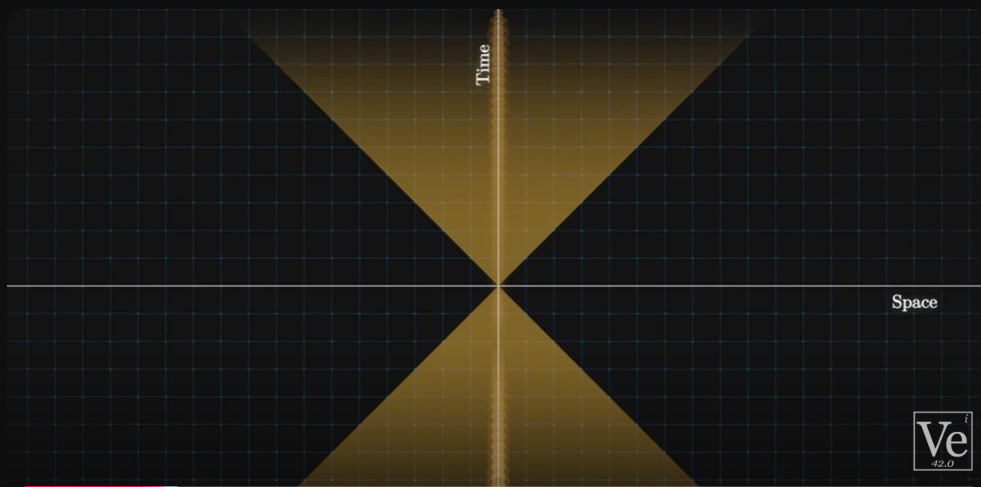
\includegraphics[width=0.8\textwidth]{graph}\\
\end{center}

that is what eistiens equations explain how to calculate separation between two events in curved geometry of space time.
\begin{center}
    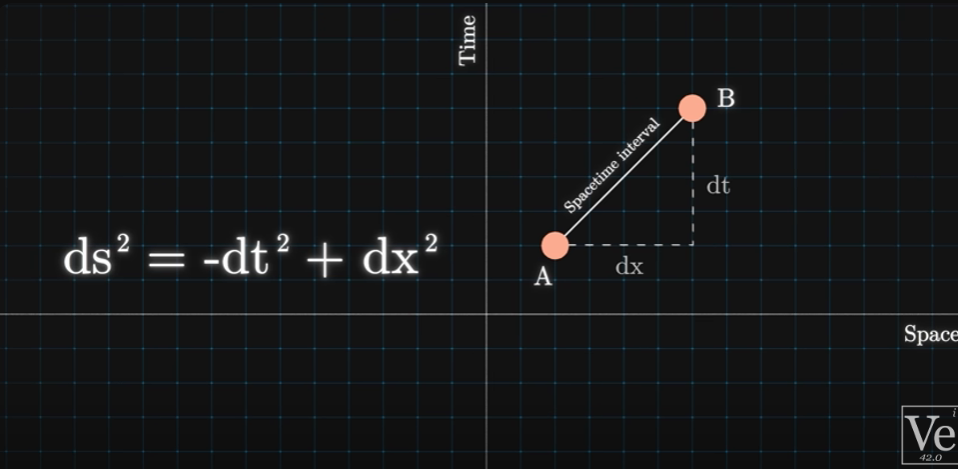
\includegraphics[width=0.8\textwidth]{graph2}\\
\end{center}

\section{ Schwarzschild equation}
\[
ds^2 = -\left(1 - \frac{R_s}{r}\right) dt^2 + \left(\frac{1}{1 - \frac{R_s}{r}}\right) dr^2 + r^2 d\Omega^2
\]
\textbf{Explanation of Terms:}

\begin{itemize}
    \item \(\mathbf{ds^2}\): 
    This represents the infinitesimal spacetime interval between two events. It incorporates both time (\(t\)) and space (\(r\), angular components) measurements.
    
    \item \(\mathbf{R_s}\) (\textit{Schwarzschild radius}): 
    \[
    R_s = \frac{2GM}{c^2}
    \]
    where \(G\) is the gravitational constant, \(M\) is the mass of the central object, and \(c\) is the speed of light. This radius defines the event horizon of a black hole; inside this radius, nothing can escape the black hole's gravity.
    
    \item \(\mathbf{t}\) (\textit{Time coordinate}): 
    Represents the time measured by a distant observer far away from the gravitational source.
    
    \item \(\mathbf{r}\) (\textit{Radial coordinate}): 
    Represents the distance from the center of the mass (e.g., a black hole or star). It is the radius in spherical coordinates.
    
    \item \(\mathbf{d\Omega^2}\): 
    Represents the angular part of the metric in spherical coordinates. It is given by:
    \[
    d\Omega^2 = d\theta^2 + \sin^2\theta \, d\phi^2
    \]
    where \(\theta\) is the polar angle and \(\phi\) is the azimuthal angle.

    \item \textbf{The terms:}
    \begin{itemize}
        \item \(-\left(1 - \frac{R_s}{r}\right) dt^2\): This factor shows how time slows down near the gravitational source (\textit{gravitational time dilation}).
        \item \(\left(\frac{1}{1 - \frac{R_s}{r}}\right) dr^2\): This term describes how distances in the radial direction are stretched as you approach the Schwarzschild radius.
        \item \(r^2 d\Omega^2\): This term describes the geometry of a sphere (the surface area and angular measurements) around the mass at radius \(r\).
    \end{itemize}
\end{itemize}

The Schwarzschild radius marks the point where gravity becomes so strong that the escape velocity exceeds the speed of light. Once an object is compressed within this radius, nothing—not even light—can escape, creating a black hole. These objects are completely dark, swallowing up all matter and light that crosses their boundary, known as the event horizon. For such an extreme phenomenon to occur, an immense amount of mass must be compressed into an incredibly small space, making black holes seem impossible to exist—at least initially.

However, the study of dying stars revealed how black holes could form naturally. When massive stars exhaust their nuclear fuel, gravity overwhelms the pressure supporting the star, causing it to collapse. For stars with enough mass, this collapse continues until it forms a singularity—a point of infinite density—surrounded by an event horizon at the Schwarzschild radius. What was once theoretical became reality through observations of supernovae and the effects of black holes on nearby objects, confirming their existence as a natural consequence of the universe's most massive stars.

\section{Entry of Chandrashekar and his Explanation of existance of black holes}
During a star's life, it maintains a delicate balance between two opposing forces: the inward pull of gravity and the outward push of radiation pressure generated by nuclear fusion in its core. Fusion releases enormous energy that counteracts gravity, preventing the star from collapsing. However, when the star exhausts its nuclear fuel, the fusion process stops, causing the radiation pressure to drop. Gravity, now unopposed, pulls all the material of the star inward toward its center.

As the collapse begins, electrons and fermions (particles that make up matter) resist being squeezed into the same space due to the Pauli Exclusion Principle, which states that no two fermions can occupy the same quantum state. This resistance creates electron degeneracy pressure, a quantum effect that prevents the star from collapsing completely. This pressure stabilizes smaller stars, such as white dwarfs, against further collapse.

Indian astrophysicist Subrahmanyan Chandrasekhar discovered a critical limit to this phenomenon, now known as the Chandrasekhar Limit. He showed that if the mass of the collapsing star exceeds about 1.4 times the mass of the Sun, electron degeneracy pressure is no longer sufficient to resist gravity. Beyond this point, electrons are forced to combine with protons, creating neutrons and releasing neutrinos in the process.

The resulting star, composed mostly of densely packed neutrons, is called a neutron star. Neutrons, being far more massive than electrons (about 2,000 times), provide a much stronger degeneracy pressure, allowing them to resist further collapse. This discovery not only explained the formation of neutron stars but also highlighted the incredible power of quantum mechanics in shaping the fate of dying stars.

\section{New perspective of Black hole}
\begin{center}
    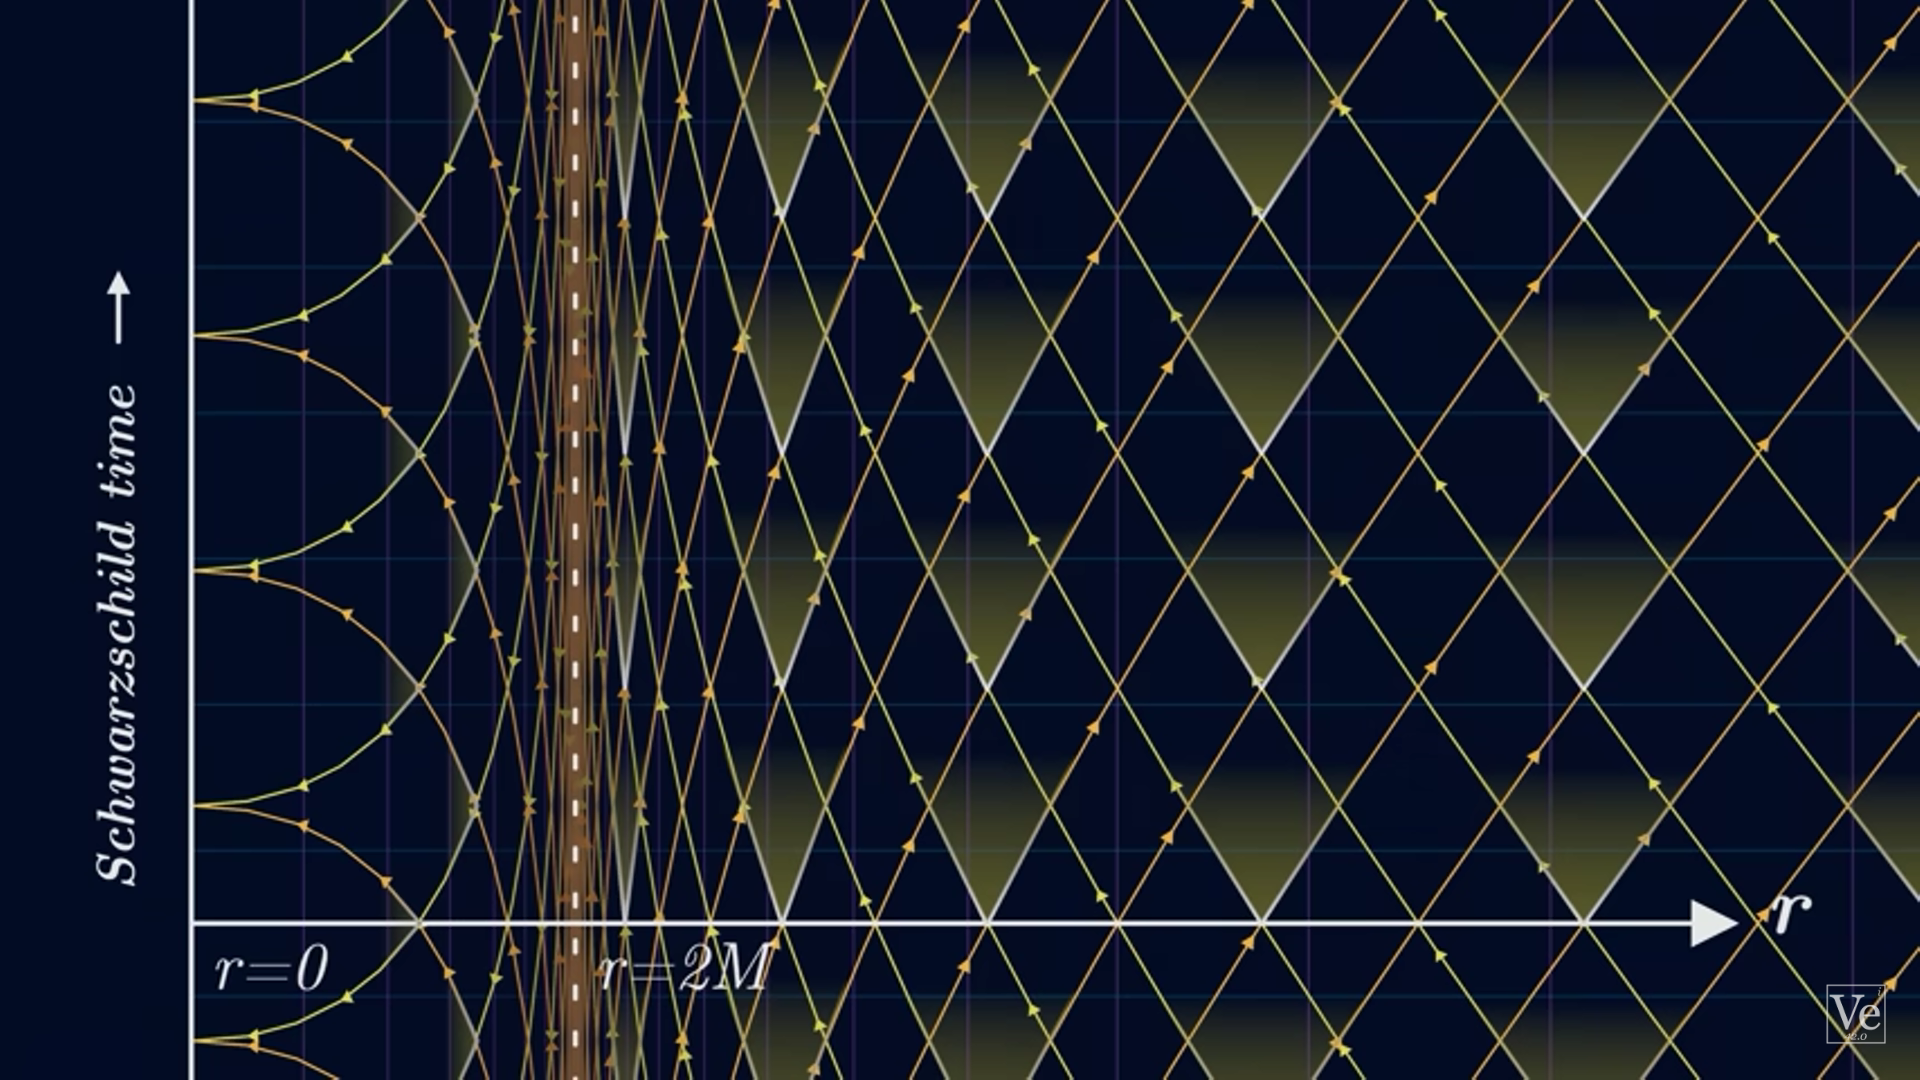
\includegraphics[width=0.8\textwidth]{Screenshot (473)}\\
\end{center}

Imagine a black hole as a cosmic waterfall, where the flow of water represents the flow of spacetime itself. Far away from the center, the current is gentle, and objects (like photons or particles) can swim against it with relative ease. However, as you move closer to the center, the current becomes faster and stronger, making it increasingly difficult for anything to escape.

At a certain point, known as the \textit{event horizon}, the current of spacetime flows so fast that even light (the fastest thing in the universe) cannot swim against it. Photons near this horizon are moving as fast as they possibly can, but they are just barely holding their position or falling inward. This is the boundary where the escape velocity equals the speed of light. Beyond this point, the flow of spacetime becomes faster than the speed of light, and nothing—neither light nor matter—can escape.

From the perspective of someone watching from outside the black hole, objects falling into the black hole appear to slow down as they approach the event horizon. This happens because of \textit{gravitational time dilation}, where time slows down in stronger gravitational fields. To the distant observer, the object never truly crosses the horizon but instead appears frozen in time at the edge, fading out as the light it emits is stretched to longer and longer wavelengths (\textit{gravitational redshift}). The last visible photon from the object comes from just outside the event horizon, making it impossible to observe anything beyond this boundary.

Thus, the waterfall analogy helps us understand why the black hole is a one-way region—beyond the event horizon, the "current" of spacetime flows faster than light, ensuring that nothing can escape, and for distant observers, the black hole appears as a dark void with no way to see inside.
\[
t_{ff} = t + 2\sqrt{2Mr} + 2M \ln \left| \frac{\sqrt{r} - \sqrt{2M}}{\sqrt{r} + \sqrt{2M}} \right|
\]

\textbf{Explanation of the Equation:}

\begin{itemize}
    \item \(\mathbf{t_{ff}}\): This represents the \textit{coordinate time} that it takes for an object to free-fall from a radial distance \(r\) to the Schwarzschild radius in the frame of a distant observer. 
    \item \(\mathbf{t}\): The \textit{proper time}, which is the time experienced by an observer close to the falling object.
    \item \(\mathbf{\sqrt{2Mr}}\): This term comes from the Schwarzschild solution and represents the contribution of radial distance and mass \(M\) to the free-fall time. Here, \(M\) is the mass of the black hole.
    \item \(\mathbf{\ln \left| \frac{\sqrt{r} - \sqrt{2M}}{\sqrt{r} + \sqrt{2M}} \right|}\): This logarithmic term captures the effects of spacetime curvature as the object approaches the event horizon. It accounts for the fact that, from the perspective of a distant observer, the object appears to slow down infinitely as it nears the Schwarzschild radius.
    
\end{itemize}


\end{document}




